\chapter{Algoritmi}\label{algoritmi}

\section{Notazione}\label{notazione}

La notazione utilizzata è la seguente:

\begin{itemize}
    \item \textit{user}: l'utente/i
    \item \textit{item}: l'elemento/i
    \item \textit{rating}: valutazione/i
    \item $m$: numero di \textit{user}
    \item $n$: numero di \textit{item}
    \item $R$: l'insieme di tutti i \textit{rating}/interazioni.
    \item $R_{train}$, $R_{test}$ e $\hat{R}$ indicano il \textit{training set}, il \textit{test set} e l'insieme dei \textit{rating} previsti.
    \item $U$ : l'insieme di tutti gli \textit{user}. $u$ e $v$ indicano gli \textit{user}.
    \item $I$ : l'insieme di tutti gli \textit{item}. $i$ e $j$ indicano gli \textit{item}.
    \item $U_i$ : l'insieme di tutti gli \textit{user} che hanno valutato l'\textit{item} $i$.
    \item $U_{ij}$ : l'insieme di tutti gli \textit{user} che hanno valutato sia l'\textit{item} $i$ che l'\textit{item} $j$.
    \item $I_u$ : l'insieme di tutti gli \textit{item} valutati dallo \textit{user} $u$.
    \item $I_{uv}$ : l'insieme di tutti gli \textit{item} valutati sia dallo \textit{user} $u$ che dallo \textit{user} $v$.
    \item $r_{ui}$ : il \textit{rating} \textit{vero} dello \textit{user} $u$ per l'\textit{item} $i$.
    \item $\hat{r}_{ui}$ : il \textit{rating} \textit{stimato} dello \textit{user} $u$ per l'\textit{item} $i$.
    \item $b_{ui}$ : il \textit{rating} di base dello \textit{user} $u$ per l'\textit{item} $i$.
    \item $\mu$ : la media di tutti i \textit{rating}.
    \item $\mu_u$ : la media di tutti i \textit{rating} dati dallo \textit{user} $u$.
    \item $\mu_i$ : la media di tutti i \textit{rating} date all'\textit{item} $i$.
    \item $\sigma_u$ : la deviazione standard di tutti i \textit{rating} dati dallo \textit{user} $u$.
    \item $\sigma_i$ : la deviazione standard di tutte le valutazioni date all'\textit{item} $i$.
    \item $N_i^k(u)$ : i $k$ vicini più prossimi dello \textit{user} $u$ che hanno valutato l'\textit{item} $i$. Questo insieme è calcolato utilizzando una metrica di similarità.
    \item $N_u^k(i)$ : i $k$ vicini più prossimi dell'\textit{item} $i$ che sono valutati dallo \textit{user} $u$. Questo insieme è calcolato utilizzando una metrica di similarità.
    \item $\gamma$: iperparametro, il \textit{learning rate} utilizzato per l'algoritmo SGD.
    \item $\lambda$: iperparametro, corrisponde al fattore di regolarizzazione nella funzione obbiettivo
    \item $\hat{x}_{uij}$: score che rappresenta la preferenza dello \textit{user} \textit{i} per l'\textit{item} \textit{i} rispetto all'\textit{item} \textit{j}
    \item $N$: numero di epoche per l'algoritmo \textit{Gradient Descent}.
\end{itemize}

\section{Algoritmi per il feedback esplicito}\label{algoritmi-per-feedback-esplicito}

\subsection{SVD}\label{svd}

L'algoritmo SVD (\textit{singular value decomposition}), è stato reso popolare da Simon Funk durante la competizione \textit{the Netflix Prize} dimostrando come modelli di fattorizzazione matriciale sono superiori alle tecniche classiche basate su \textit{nearest neighbor}\ref{knn} per
la produzione di raccomandazioni.

I modelli di \textit{matrix factorization} mappano gli \textit{user} e gli \textit{item} in uno spazio latente comune di dimensione $k$, che rappresenta il numero di caratteristiche latenti. Ogni \textit{item} $i$ è associato a un vettore $q_i$ di dimensione $k$, che misura quanto l'\textit{item} possieda ciascuna di queste caratteristiche latenti. Per ogni \textit{user} $u$, invece, il vettore $p_u$ misura l'interesse dello \textit{user} per gli \textit{item}. Il numero di fattori è un iperparametro dell'algoritmo.

In questo spazio, le interazioni tra \textit{user} e \textit{item} vengono modellate come prodotti scalari tra i rispettivi vettori. Lo spazio latente cerca di spiegare i \textit{rating} caratterizzando sia gli \textit{item} che gli textit{user} in base a fattori che vengono automaticamente dedotti. Ad esempio, se gli \textit{item} sono film, i fattori potrebbero appresentare il genere piuttosto che un altro (e.g. Azione contro Drama), profondità della trama o il concetto di ``adatto ai bambini".

Il prodotto scalare risultante cattura l'interazione tra lo \textit{user} $u$ e l'\textit{item} $i$, che corrisponde all'interesse complessivo dello \textit{user} per le caratteristiche dell'\textit{item}. Il \textit{rating} finale viene ottenuto aggiungendo anche i predittori di base sopra menzionati, che dipendono solo dallo \textit{user} o dall'\textit{item}. Pertanto, un \textit{rating} viene predetto dalla regola~\cite{SVD_analysis}~\cite{Recommendation_book}:

\[
\hat{r}_{ui} = \mu + b_u + b_i + q_i^T p_u
\]

Dove:
\begin{itemize}
    \item $ b_u $ e $ b_i $ sono i bias dello \textit{user} $u$ e dell'\textit{item} $i$ rispettivamente. Sono una sorta di correzione basata sull'effetto dello \textit{user} e dell'\textit{item}.
    \item $ q_i^T p_u $ è il prodotto interno tra i vettori latenti dello \textit{user} e dell'\textit{item}.
\end{itemize}

Se lo \textit{user} $u$ è sconosciuto, allora il bias $b_u$ e i fattori $p_u$ vengono considerati uguali a zero. Lo stesso vale per
l'\textit{item} $i$, con $b_i$ e $q_i$ anch'essi assunti uguali a zero.

Per apprendere i parametri del modello ($b_u$, $b_i$, $p_u$, $q_i$), si minimizza l'errore quadratico regolarizzato tra le \textit{rating} reali e quelle previste. L'errore quadratico è dato da:

\[
\min \sum\limits_{(u,i) \in K} \left( (r_{ui} - \hat{r}_{ui})^2 + \lambda (\|q_i\|^2 + \|p_u\|^2 + b_u^2 + b_i^2) \right)
\]


Dove il primo termine è l'errore quadratico tra le \textit{rating} previste e reali e il secondo termine è la regolarizzazione, che penalizza valori troppo grandi per i parametri $b_u$, $b_i$, $p_u$, $q_i$ per evitare l'overfitting.

Per ottimizzare questi parametri, viene usata la \textit{Stochastic Gradient Descent} (SGD), che aggiorna i parametri dopo ogni  esempio di training (ad esempio, per ogni \textit{rating} di un \textit{user}).

Per ogni \textit{rating} ($r_{ui}$) data, viene fatta una previsione ($\hat{r}_{ui}$), e l'errore di previsione associato ($e_{ui} = r_{ui} - \hat{r}_{ui}$) viene calcolato. Per un dato caso di \textit{addestramento} ($r_{ui}$), modifichiamo i parametri spostandoci nella
direzione opposta al gradiente, ottenendo:

\begin{itemize}
    \item $b_u \leftarrow b_u + \gamma \cdot e_{ui}$
    \item $b_i \leftarrow b_i + \gamma \cdot e_{ui}$
    \item $q_i \leftarrow q_i + \gamma \cdot e_{ui} \cdot p_u$
    \item $p_u \leftarrow p_u + \gamma \cdot e_{ui} \cdot q_i$
\end{itemize}

Queste formule vengono utilizzate per aggiornare i parametri durante l'addestramento del modello, in modo da ridurre l'errore tra le
\textit{rating} reali e quelle previste.

Per ottenere un ulteriore miglioramento, si possono applicare $\gamma$ e $\lambda$ separati per i bias degli \textit{user}, i bias degli
\textit{item} e i fattori stessi~\cite{SVD_optimized}.

I punti di forza dell'algoritmo sono:

\begin{itemize}
    \item semplicità: l'algoritmo SVD è relativamente semplice da comprendere e implementare.
    \item riduzione della dimensionalità: l'algoritmo permette di ridurre la dimensione del problema mappando sia gli \textit{user} che gli \textit{item} in uno spazio latente di dimensione inferiore, gestendo la sparsità delle matrici. Funziona molto bene quando la matrice delle valutazioni è abbastanza completa. 
    \item caratteristiche latenti: identifica strutture sottostanti che non sono immediatamente evidenti.
\end{itemize}

L'algoritmo soffre anche di diverse problematiche:

\begin{itemize}
    \item problemi con la sparsità: può produrre raccomandazioni imprecise quando la matrice delle valutazioni è troppo sparsa, perché la decomposizione non riesce a estrarre informazioni significative. 
    \item non tiene conto di informazioni aggiuntive: non considera altri fattori come informazioni temporali, contenuti aggiuntivi sugli \textit{item} o preferenze esplicite/implicite dello \textit{user} che non sono registrati nella matrice.
    \item computazionalmente costosa: la decomposizione di una matrice grande è costosa in termini di tempo e risorse.
    \item overfitting: se non adeguatamente regolarizzato si rischia l'overfitting.
\end{itemize}

\subsection{SVD\protect++}

La precisione delle previsioni può essere migliorata considerando anche il feedback implicito, che fornisce un'indicazione aggiuntiva delle preferenze degli \textit{user}. Questo è particolarmente utile per gli \textit{user} che hanno fornito molto più feedback implicito che esplicito. Anche nei casi in cui il feedback implicito indipendente è assente, è possibile catturare un segnale significativo tenendo conto degli \textit{item} che gli \textit{user} hanno valutato, indipendentemente dal valore del \textit{rating}. Ciò ha portato a diversi metodi (\textit{Asymmetric-SVD}, \textit{SVD++}, \textit{SVD\_KNN}, ecc.~\cite{SVD++, SVD_KNN}) che modellano il fattore \textit{user} in base agli \textit{item} valutati. Il metodo \textit{SVD++} ha dimostrato di offrire una precisione superiore rispetto a \textit{SVD}.

Viene aggiunto un secondo set di fattori degli \textit{item}, che collega ogni \textit{item} $i$ a un vettore di fattori $y_i$ di dimensione $k$. Questi nuovi fattori vengono utilizzati per caratterizzare gli \textit{user} in base al set di \textit{item} che hanno valutato. La nuova predizione si calcola come segue:

\[
\hat{r}_{ui} = \mu + b_u + b_i + q_i^T \left(p_u + |I_u|^{\frac{1}{2}} \sum\limits_{j \in I_u} y_j \right)
\]

Ora, un \textit{user} $u$ viene modellato come $p_u + |I_u|^{\frac{1}{2}} \sum\limits_{j \in I_u} y_j$, mentre la parte $\sum\limits_{j \in I_u} y_j$ rappresenta i feedback impliciti. Poiché i vettori $y_j$ sono centrati intorno a zero grazie alla regolarizzazione $|I_u|^{\frac{1}{2}}$, la varianza rispetto all'intervallo di valori osservati $|I_u|$ viene stabilizzata.

I parametri del modello vengono determinati minimizzando la funzione di errore quadratico regolarizzato, utilizzando sempre \textit{stochastic gradient descent}. Si itera su tutti i \textit{rating}:

\begin{itemize}
  \item $b_u \leftarrow b_u + \gamma \cdot (e_{ui} - \lambda \cdot b_u)$
  \item $b_i \leftarrow b_i + \gamma \cdot (e_{ui} - \lambda \cdot b_i)$
  \item $q_i \leftarrow q_i + \gamma \cdot \left( e_{ui} \cdot \left( p_u + |I_u|^{-\frac{1}{2}} \sum\limits_{j \in I_u} y_j \right) - \lambda \cdot q_i \right)$
  \item $p_u \leftarrow p_u + \gamma \cdot (e_{ui} \cdot q_i - \lambda \cdot p_u)$
  \item $\forall j \in I_u: \quad y_j \leftarrow y_j + \gamma \cdot \left( e_{ui} \cdot |I_u|^{-\frac{1}{2}} \cdot q_i - \lambda \cdot y_j \right)$
\end{itemize}

È possibile introdurre diversi tipi di feedback implicito nel modello simultaneamente, utilizzando set aggiuntivi di fattori degli \textit{item}.

I punti di forza dell'algoritmo sono:

\begin{itemize}
    \item miglioramento della personalizzazione: SVD++ è un miglioramento significativo rispetto a SVD, poiché prende in considerazione anche l'influenza degli \textit{item} che lo \textit{user} ha già valutato nel termine $\sum\limits_{j \in I_u} y_j$, il che lo rende molto più sensibile alle preferenze individuali dello \textit{user}.
    \item migliore gestione della sparsità: poiché SVD++ tiene conto dei feedback impliciti, riesce a fare previsioni migliori anche quando la matrice delle valutazioni è sparsa.
    \item previsioni più accurate: i feedback impliciti aiutano a produrre previsioni più accurate, soprattutto in scenari dove gli \textit{user} hanno interagito con più \textit{item}.
\end{itemize}

L'algoritmo soffre anche di diverse problematiche:

\begin{itemize}
    \item complessità computazionale maggiore: la necessità di aggiornare $y_i$ aumenta il carico computazionale.
    \item richiede più dati: poiché prende in considerazione anche i feedback impliciti, ha bisogno di un numero maggiore di dati per generare previsioni precise.
    \item overfitting: SVD++ è più propenso a overfitting su dataset piccoli.
\end{itemize}

\subsection{NMF}\label{nmf}

Un algoritmo di \textit{collaborative filtering} basato sulla \textit{fattorizzazione matriciale non negativa}.  

Questo algoritmo è molto simile a SVD\ref{svd} ma con una restrizione che tutti gli elementi devono essere non negativi. Questo ha senso, ad esempio, quando si tratta di rating o quantità (che non possono essere negativi).

L'idea è approssimare la matrice $R$ come prodotto di due matrici più piccole:

\[
R \approx WH
\]

dove:
\begin{itemize}
    \item $W \in \mathbb{R}_{\geq 0}^{m \times k}$ rappresenta la matrice dei profili latenti degli \textit{user};
    \item $H \in \mathbb{R}_{\geq 0}^{k \times n}$ rappresenta la matrice dei profili latenti degli \textit{item};
    \item $k$ è il numero di fattori latenti e iperparametro dell'algoritmo
\end{itemize}

Il \textit{rating} stimato dello \textit{user} $u$ per l'\textit{item} $i$ è calcolato come~\cite{NMF2}~\cite{NMF3}:

\[
\hat{r}_{ui} = \sum_{f=1}^k W_{uf} H_{fi} = q_i^T p_u
\]

dove i fattori \textit{user} e articolo vengono mantenuti positivi

L'obiettivo di apprendimento è minimizzare l'errore quadratico sui \textit{rating} osservati nel \textit{training set} $R_{train}$:

\[
\min_{W, H} \sum_{(u,i) \in R_{train}} \left( r_{ui} - \hat{r}_{ui} \right)^2 \quad \text{s.t.} \quad W \geq 0,\ H \geq 0
\]

In forma matriciale, questo si può esprimere come:

\[
\min_{W, H} \ \| R_{train} - WH \|_F^2 \quad \text{con} \quad W \geq 0,\ H \geq 0
\]

dove $\| \cdot \|_F$ è la norma di Frobenius.

La procedura di ottimizzazione è una SGD regolarizzata~\cite{NMF} con una scelta specifica della dimensione del passo che garantisce la non negatività dei fattori, a condizione che anche i loro valori iniziali siano positivi.

A ogni iterazione i fattori vengono aggiornati come segue:

\begin{equation}
    \begin{split}
        p_{uf} &\leftarrow p_{uf} \cdot \frac{\sum\limits_{i \in I_u} q_{if} \cdot r_{ui}}{\sum\limits_{i \in I_u} q_{if} \cdot \hat{r}_{ui} + \lambda_u |I_u| p_{uf}}\\
        q_{if} &\leftarrow q_{if} \cdot \frac{\sum\limits_{u \in U_i} p_{uf} \cdot r_{ui}}{\sum\limits_{u \in U_i} p_{uf} \cdot \hat{r}_{ui} + \lambda_i |U_i| q_{if}}
    \end{split}
\end{equation}

Questo algoritmo è altamente dipendente dai valori iniziali con cui vengono inizializzate le matrici $H$ e $W$. I fattori latenti degli \textit{user} e degli \textit{item} vengono inizializzati casualmente in modo uniforme tra un minimo e un massimo, solitamente nell'intervallo $[0, 1]$.

Gli iper-parametri $\lambda_u$ e $\lambda_i$ corrispondono alla regolarizzazione rispettivamente per \textit{user} e \textit{item}.

Anche in questo caso si può utilizzare la predizione con l'utilizzo di baseline\ref{svd}.

\[
\hat{r}_{ui} = \mu + b_u + b_i + q_i^T p_u
\]

garantendo comunque fattori positivi. Le baselines sono ottimizzate nello stesso modo dell'algoritmo SVD. Pur producendo una migliore accuratezza, la versione che utilizza baseline sembra molto incline all'overfitting, che può essere ridotto diminuendo $k$ o aumentando la regolarizzazione.

NFM, grazie al vincolo della non negatività, è più interpretabile di SVD: i valori nelle matrici fattorizzate $W$ e $H$ sono tutti $\geq 0$, quindi possono essere interpretati come pesi o intensità (es. quanto uno \textit{user} apprezza un certo genere, quanto un \textit{item} rappresenta un tema).

L'algoritmo soffre anche di diverse problematiche:

\begin{itemize}
    \item dipendenza dall'inizializzazione: l'algoritmo può convergere a minimi locali diversi a seconda dei valori iniziali, e non garantisce una soluzione unica o ottima
    
    \item non adatta per dati con valori negativi: NMF non può gestire valori negativi nei dati di input, a differenza di SVD
    
    \item convergenza più lenta: rispetto ad altri metodi la convergenza può essere più lenta e richiede tuning di più parametri
    \item mancanza di soluzione chiusa: SVD può gestire valori negativi e ha una soluzione ottima in termini di errore quadratico minimo
\end{itemize}

\subsection{KNN (K-Nearest Neighbors)}\label{knn}
Si tratta di algoritmi derivati direttamente da un approccio di base basato sui \textit{nearest neighbors}.

Gli algoritmi ispirati al KNN (\textit{K Nearest Neighbors}) sono una classe di algoritmi di \textit{recommendation} che si basano sull'idea che gli \textit{user} simili tendono a valutare gli stessi \textit{item} in modo simile. Questi algoritmi sono semplici da implementare e possono essere molto efficaci per problemi a piccola scala.

Il numero effettivo di vicini che vengono considerati per calcolare la predizione è minore o uguale a $k$: potrebbero non esserci abbastanza vicini e/o gli insiemi $N_i^k(u)$ e $N_u^k(i)$ includono solo vicini per i quali la misura di similarità è positiva (non avrebbe senso considerare \textit{user} o \textit{item} correlati negativamente).

$k$ è un iperparametro di ciascun algoritmo.

Alcune misure di similarità, sia per \textit{user} che per \textit{item}, sono:
\begin{itemize}
    \item Coseno:
        \[
        \text{cosine sim}(u, v) = \frac{\sum\limits_{i \in I_{uv}} r_{ui} \cdot r_{vi}}{\sqrt{\sum\limits_{i \in I_{uv}} r_{ui}^2} \cdot \sqrt{\sum\limits_{i \in I_{uv}} r_{vi}^2}}
        \]
        oppure
        \[
        \text{cosine sim}(i, j) = \frac{\sum\limits_{u \in U_{ij}} r_{ui} \cdot r_{uj}}{\sqrt{\sum\limits_{u \in U_{ij}} r_{ui}^2} \cdot \sqrt{\sum\limits_{u \in U_{ij}} r_{uj}^2}}
        \]
    \item \textit{Mean Square Difference} (MSD):
        \[
        \text{msd}(u, v) = \frac{1}{|I_{uv}|} \cdot \sum\limits_{i \in I_{uv}} (r_{ui} - r_{vi})^2
        \]
        oppure
        \[
        \text{msd}(i, j) = \frac{1}{|U_{ij}|} \cdot \sum\limits_{u \in U_{ij}} (r_{ui} - r_{uj})^2
        \]
        La similarità è calcolata come:
        \begin{align*}
            \text{msd sim}(u, v) &= \frac{1}{\text{msd}(u, v) + 1} \\
            \text{msd sim}(i, j) &= \frac{1}{\text{msd}(i, j) + 1}
        \end{align*}
        Il termine $+1$ viene aggiunto per evitare divisioni per zero.
    \item Pearson: Il coefficiente di correlazione di Pearson può essere visto come una similarità del coseno centrato sulla media. Se non ci sono \textit{item} comuni, la similarità è 0 (non -1).
        \[
        \text{pearson sim}(u, v) = \frac{\sum\limits_{i \in I_{uv}} (r_{ui} - \mu_u) \cdot (r_{vi} - \mu_v)}{\sqrt{\sum\limits_{i \in I_{uv}} (r_{ui} - \mu_u)^2} \cdot \sqrt{\sum\limits_{i \in I_{uv}} (r_{vi} - \mu_v)^2}}
        \]
        oppure
        \[
        \text{pearson sim}(i, j) = \frac{\sum\limits_{u \in U_{ij}} (r_{ui} - \mu_i) \cdot (r_{uj} - \mu_j)}{\sqrt{\sum\limits_{u \in U_{ij}} (r_{ui} - \mu_i)^2} \cdot \sqrt{\sum\limits_{u \in U_{ij}} (r_{uj} - \mu_j)^2}}
        \]
    \item Pearson con baseline \cite{Recommendation_book}: calcola il coefficiente di correlazione di Pearson (ridotto) tra tutte le coppie di \textit{user} (o \textit{item}) utilizzando le baseline anziché le medie. Il parametro di riduzione aiuta a evitare l'overfitting quando sono disponibili solo poche valutazioni. Se non ci sono \textit{item} comuni, la similarità è 0 (non -1). Introduce un nuovo iperparametro che corrisponde alla riduzione (o \textit{``shrinkage''}). Se impostato uguale a 0, non viene applicata nessuna riduzione.
        \[
        \text{pearson baseline sim}(u, v) = \hat{\rho}_{uv} = \frac{\sum\limits_{i \in I_{uv}} (r_{ui} - b_{ui}) \cdot (r_{vi} - b_{vi})}{\sqrt{\sum\limits_{i \in I_{uv}} (r_{ui} - b_{ui})^2} \cdot \sqrt{\sum\limits_{i \in I_{uv}} (r_{vi} - b_{vi})^2}}
        \]
        oppure
        \[
        \text{pearson baseline sim}(i, j) = \hat{\rho}_{ij} = \frac{\sum\limits_{u \in U_{ij}} (r_{ui} - b_{ui}) \cdot (r_{uj} - b_{uj})}{\sqrt{\sum\limits_{u \in U_{ij}} (r_{ui} - b_{ui})^2} \cdot \sqrt{\sum\limits_{u \in U_{ij}} (r_{uj} - b_{uj})^2}}
        \]
        Il coefficiente ridotto si calcola come:
        \begin{align*}
            \text{pearson baseline shrunk sim}(u, v) &= \frac{|I_{uv}| - 1}{|I_{uv}| - 1 + \text{shrinkage}} \cdot \hat{\rho}_{uv} \\
            \text{pearson baseline shrunk sim}(i, j) &= \frac{|U_{ij}| - 1}{|U_{ij}| - 1 + \text{shrinkage}} \cdot \hat{\rho}_{ij}
        \end{align*}
        Per il calcolo della baseline, si consideri la parte di \ref{knn_baseline}.
\end{itemize}

Altro iperparametro da considerare è il supporto minimo, che corrisponde al numero minimo di \textit{item} in comune o il numero minimo di \textit{user} in comune affinché la similarità non sia zero, i.e., se $|I_{uv}| < \text{min support}$, allora $\text{sim}(u, v) = 0$. Lo stesso vale per gli \textit{item}.

\subsubsection{KNN base}

L'algoritmo KNN base è l'algoritmo più semplice. Prevede il  \textit{rating} di un \textit{user} $u$ per un \textit{item} $i$ come la media ponderata dei \textit{rating} degli $k$ vicini più simili di $u$ o $i$, a seconda che si utilizzi un approccio basato sugli \textit{user} o sugli \textit{item}.

La predizione viene calcolata come:

\[
\hat{r}_{ui} = \frac{\sum\limits_{v \in N^k_i(u)} \text{sim}(u, v) \cdot r_{vi}}{\sum\limits_{v \in N^k_i(u)} \text{sim}(u, v)}
\]

oppure

\[
\hat{r}_{ui} = \frac{\sum\limits_{j \in N^k_u(i)} \text{sim}(i, j) \cdot r_{uj}}{\sum\limits_{j \in N^k_u(i)} \text{sim}(i, j)}
\]

dipendentemente dall'approccio utilizzato.

\subsubsection{KNN con la media}
\label{algoritmo-knn-con-la-media}

L'algoritmo è una variante dell'algoritmo KNN base che tiene conto della media dei \textit{rating} degli \textit{user} o degli \textit{item}.

La predizione viene calcolata come:

\[
\hat{r}_{ui} = \mu_u + \frac{\sum\limits_{v \in N_k(u)} \text{sim}(u, v) \cdot (r_{vi} - \mu_v)}{\sum\limits_{v \in N_k(u)} \text{sim}(u, v)}
\]

oppure

\[
\hat{r}_{ui} = \mu_i + \frac{\sum\limits_{j \in N^k_u(i)} \text{sim}(i, j) \cdot (r_{uj} - \mu_j)}{\sum\limits_{j \in N^k_u(i)} \text{sim}(i, j)}
\]

dipendentemente dall'approccio utilizzato.

\subsubsection{KNN normalizzato}
\label{algoritmo-knn-normalizzato}

L'algoritmo è una variante dell'algoritmo che utilizza la media con l'aggiunta della normalizzazione \textit{z-score}, con la deviazione standard dello \textit{user} o dell'\textit{item}, dei \textit{rating} corrispondenti prima di calcolare la similarità.

La predizione viene calcolata come:

\[
\hat{r}_{ui} = \mu_u + \sigma_u \frac{\sum\limits_{v \in N^k_i(u)} \text{sim}(u, v) \cdot (r_{vi} - \mu_v) / \sigma_v}{\sum\limits_{v \in N^k_i(u)} \text{sim}(u, v)}
\]

oppure

\[
\hat{r}_{ui} = \mu_i + \sigma_i \frac{\sum\limits_{j \in N^k_u(i)} \text{sim}(i, j) \cdot (r_{uj} - \mu_j) / \sigma_j}{\sum\limits_{j \in N^k_u(i)} \text{sim}(i, j)}
\]

dipendentemente dall'approccio utilizzato.

\subsubsection{KNN con baseline}\label{knn_baseline}
\label{knn-con-baseline}

L'algoritmo KNN con baseline \cite{KNN_baseline} è una variante dell'algoritmo base che tiene conto degli effetti di bias degli \textit{user} o degli \textit{item}.

La predizione viene calcolata come:

\[
\hat{r}_{ui} = b_{ui} + \frac{\sum\limits_{v \in N^k_i(u)} \text{sim}(u, v) \cdot (r_{vi} - b_{vi})}{\sum\limits_{v \in N^k_i(u)} \text{sim}(u, v)}
\]

oppure

\[
\hat{r}_{ui} = b_{ui} + \frac{\sum\limits_{j \in N^k_u(i)} \text{sim}(i, j) \cdot (r_{uj} - b_{uj})}{\sum\limits_{j \in N^k_u(i)} \text{sim}(i, j)}
\]

dipendentemente dall'approccio utilizzato.

La baseline $b_{ui}$ viene calcolata come:

\[
b_{ui} = \mu + b_u + b_i
\]

Per calcolare $b_u$ e $b_i$, occorre minimizzare il seguente errore quadratico regolarizzato:

\[
\sum\limits_{r_{ui} \in R_{train}} \left(r_{ui} - \mu + b_u + b_i\right)^2 + \lambda \left(b_u^2 + b_i^2 \right).
\]

Il termine di regolarizzazione $\lambda \left(b_u^2 + b_i^2 \right)$ serve per evitare l'overfitting penalizzando la grandezza dei parametri.

La minimizzazione può essere effettuata tramite \textit{Stochastic Gradient Descent} o \textit{Alternating Least Squares}.

Per \textit{Alternating Least Squares}, i due valori di $b_u$ e $b_i$ si ottengono come:

\[
b_i = \frac{\sum\limits_{r_{ui} \in R_{train}} (r_{ui} - \mu)}{\lambda_2 + |U_i|}
\]

e

\[
b_u = \frac{\sum\limits_{r_{ui} \in R_{train}} (r_{ui} - \mu - b_i)}{\lambda_3 + |I_u|}
\]

I punti di forza della famiglia di algoritmi KNN sono:
\begin{itemize}
    \item semplicità: Gli algoritmi KNN sono facili da capire e implementare. L'idea di base di trovare ``vicini" simili è intuitiva e facilmente comprensibile.
    \item nessuna assunzione sui dati: l'algoritmo non fa assunzioni sulla distribuzione dei dati. Questo lo rende flessibile e adatto a una varietà di dataset.
    \item aggiornamento: l'aggiunta di nuovi dati non richiede una fase di addestramento esplicita. Questo lo rende utile in ambienti in cui i dati cambiano frequentemente o per previsioni online.
    \item flessibilità: KNN può essere utilizzato sia per problemi di \textit{recommendation} basati su \textit{user} che basati su \textit{item}.
\end{itemize}

Gli algoritmi soffrono anche di diverse problematiche:
\begin{itemize}
    \item costo computazionale: KNN può essere computazionalmente costoso, soprattutto con set di dati di grandi dimensioni.
    \item requisiti di memoria: KNN richiede la memorizzazione dell'intero set di dati, il che può essere problematico per set di dati molto grandi.
    \item sensibilità alla scelta di $k$: La scelta del valore di k può avere un impatto significativo sulle prestazioni di KNN. Un valore di k troppo piccolo può portare a un overfitting, mentre un valore di k troppo grande può portare a un underfitting. Inoltre, la ricerca dei $k$ vicini più prossimi richiede il calcolo delle distanze tra tutti i punti dati.
    \item gestione della sparsità dei dati: la sparsità può rendere difficile trovare vicini significativi e quindi portare a raccomandazioni di bassa qualità.
\end{itemize}

\subsection{CoClustering}\label{coclustering}

La soluzione proposta da Thomas George e Srujana Merugu~\cite{Co-Clustering} utilizza il \textit{co-clustering}. Questa tecnica viene utilizzata per raggruppare simultaneamente due entità in un dataset. Nel caso di un sistema di \textit{recommendation} basato su \textit{collaborative filtering}, l'obiettivo è trovare gruppi di \textit{user} simili e gruppi di \textit{item} simili. Il co-clustering cerca di partizionare simultaneamente le righe (\textit{user}) e le colonne (\textit{item}) della matrice dei \textit{rating} in modo tale che gli \textit{user} all'interno dello stesso co-cluster abbiano comportamenti di valutazione simili e \textit{item} all'interno dello stesso co-cluster siano valutati in modo simile dagli \textit{user} del co-cluster. Il numero di cluster è da definire a priori sia per gli \textit{user} che per gli \textit{item}. Il processo di co-clustering è simile al clustering tradizionale, ma mentre nel clustering classico si raggruppa solo per righe o colonne, nel co-clustering si raggruppano contemporaneamente. 

L'algoritmo, nella fase di inizializzazione, assegna casualmente i co-cluster a \textit{user} e \textit{item}. Durante l'esecuzione i co-cluster vengono aggiornati iterativamente, per cercare di migliorare la qualità del raggruppamento, alternando tra il raggruppamento degli \textit{user} e degli \textit{item} fino a convergenza. Una volta che i co-cluster sono definiti si può calcolare la media dei \textit{rating} all'interno di ciascun co-cluster. $ \overline{C_{ui}} $ rappresenta la media dei \textit{rating} all'interno del co-cluster che contiene lo \textit{user} $ u $ e l'\textit{item} $ i $. In altre parole, è il \textit{rating} medio tra gli \textit{user} e gli \textit{item} che appartengono allo stesso co-cluster.

Si può quindi definire la predizione come

\[
\hat{r}_{ui} = \overline{C_{ui}} + (\mu_u - \overline{C_u}) + (\mu_i - \overline{C_i})
\]

dove $\overline{C_u}$ è la media dei \textit{rating} del cluster di $u$ e $\overline{C_i}$ è la media dei \textit{rating} del cluster di $i$. $ \mu_u - \overline{C_u} $ e $ \mu_i - \overline{C_i} $ vengono definiti \textit{bias}. Se: 
\begin{itemize}
  \item \textit{user} mancante: la previsione è $ \overline{C_i} $
  \item \textit{item} mancante: la previsione è $ \overline{C_u} $
  \item se sia \textit{user} che \textit{item} sono mancanti: la previsione è $ \mu $, la media generale dei rating.
\end{itemize}

I punti di forza dell'algoritmo sono:

\begin{itemize}
  \item Scalabilità: l'algoritmo di co-clustering può essere facilmente parallelizzato, il che lo rende adatto per sistemi di \textit{recommendation} con grandi quantità di dati.
  \item Gestione dei comportamenti complessi: la previsione tiene conto sia del co-cluster, che considera simultaneamente i raggruppamenti di \textit{user} e \textit{item}, sia dei cluster singoli per \textit{user} e \textit{item}. Questo permette di considerare diversità e similarità sia individualmente che insieme, migliorando le previsioni.
  \item Gestione semplice degli aggiornamenti: quando nuovi dati sono aggiunti al sistema, è possibile aggiornare solo i co-cluster rilevanti senza dover ricalcolare tutto da zero. Questo è particolarmente utile per scenari dinamici e sistemi in tempo reale.
  \item Gestione della sparsità: poiché l'algoritmo raggruppa \textit{user} e \textit{item} simili, riduce l'effetto della sparsità permettendo di migliorare la qualità delle previsioni anche quando i dati disponibili sono pochi o incompleti.
\end{itemize}

L'algoritmo soffre anche di diverse problematiche:

\begin{itemize}
  \item Sensibilità ai co-cluster: la qualità delle previsioni dipende molto dal numero di co-cluster scelto e dalla loro qualità. Se il numero di co-cluster è troppo basso, il modello potrebbe non riuscire a catturare le complessità dei dati e fare previsioni imprecise. Se il numero è troppo alto, il modello potrebbe overfittare il \textit{training set}, riducendo la sua generalizzazione. Inoltre, se i co-cluster non sono ben definiti, il modello potrebbe produrre previsioni inaccurate. La scelta iniziale dei co-cluster è fondamentale. Una soluzione è quella di utilizzare l'algoritmo \textit{K-means} per definire la posizione iniziale dei cluster.
  \item Bias del co-cluster: $ \mu_u - \overline{C_u} $ e $ \mu_i - \overline{C_i} $ potrebbero non essere sempre utili in tutte le situazioni. Alcuni \textit{user} o \textit{item} potrebbero avere comportamenti che non sono ben rappresentati dai co-cluster e il modello potrebbe non adattarsi bene a queste situazioni. Ad esempio, \textit{user} che tendono a esprimere \textit{rating} bassi potrebbero non essere gestiti correttamente.
  \item Alto costo computazionale iniziale: l'algoritmo ha un alto costo computazionale durante la fase di addestramento, soprattutto con set di dati molto grandi. Anche se è scalabile, l'ottimizzazione del processo di clustering e la ricerca del numero ottimale di co-cluster richiedono parecchia computazione.
  \item Difficoltà di interpretazione: il co-clustering fornisce gruppi di \textit{user} e \textit{item} che potrebbero non essere sempre facili da interpretare o da analizzare in modo intuitivo.
\end{itemize}

Il costo computazionale per l'addestramento è $ O(W^{\text{glob}} + mkl + nkl) $ dove $ W^{\text{glob}} $ corrisponde al numero di valori diversi da 0 nella matrice in input , $l$ corrisponde al numero di cluster per gli \textit{user} e $k$ corrisponde al numero di cluster per gli \textit{item}.

Per il calcolo della predizione, il costo è $O(1)$, in quanto si tratta di operazioni media e il calcolo dei bias.

Per l'aggiornamento quando un nuovo \textit{rating} viene aggiunto o un nuovo \textit{user}/\textit{item} entra nel sistema, l'algoritmo non ricalcola tutto da zero. Invece, utilizza un aggiornamento incrementale parziale, che si basa sull'aggiornamento delle medie delle matrici:

\begin{itemize}
  \item Se il nuovo \textit{rating} riguarda un \textit{user} e un \textit{item} esistenti si aggiornano direttamente le medie.
  \item Se l'\textit{user} o l'\textit{item} è nuovo, viene assegnato temporaneamente a un co-cluster globale di transizione. Le medie vengono aggiornate e, durante la successiva esecuzione dell'algoritmo, il nuovo \textit{user}/\textit{item} viene riassegnato ai co-cluster regolari.
\end{itemize}

L'aggiornamento ha quindi costo pari a $O(1)$.

\subsection{Slope One}\label{slopeone}

L'algoritmo Slope One, introdotto da Daniel Lemire e Anna Maclachlan~\cite{SlopeOne}, è una delle soluzioni più semplici ed efficienti di collaborative filtering.
%
Le caratteristiche che lo rendono un ottimo algoritmo per la \textit{recommendation} sono:
\begin{itemize}
    \item la semplicità e facilità di implementazione
    \item velocità di calcolo: come verrà presentato più avanti alcuni valori calcolati possono essere salvati e aggiornati all'occorrenza rendendo il calcolo molto più veloce
    \item scalabilità: l'algoritmo può essere abbastanza efficace su dataset di dimensioni moderate, soprattutto se si utilizzano tecniche di compressione dei dati
    \item facilità di interpretazione
\end{itemize}
%
Viene proposto un predittore basato su differenze di \textit{rating} lineari che ha un'efficienza $O(nm)$ per predizione e $O(mn^2)$ per addestramento.

L'algoritmo si basa sulla differenza media tra le valutazioni di due \textit{item} per predire il \textit{rating} mancante. La differenza media dei \textit{rating} di due \textit{item} $i$ e $j$ viene calcolata come:

\[
    \text{dev}(i, j) = \frac{1}{|U_{i,j}|} \sum\limits_{u \in U_{i,j}} (r_{u,i} - r_{u,j})
\]

La matrice simmetrica definita da $\text{dev}(i, j)$ può essere computata una volta e aggiornata velocemente quando vengono aggiunti nuovi dati.

La predizione viene dunque calcolata come:

\[
    \hat{r}_{ui} = \mu_u + \frac{1}{|R_i(u)|} \sum\limits_{j \in R_i(u)} \text{dev}(i, j)
\]

dove:

\begin{itemize}
    \item $R_j = \{ i \mid i \in S(u), i \neq j, |S_{j,i}(\chi)| > 0 \}$ è l'insieme degli \textit{item} rilevanti
    \item $S(u)$ è il sottoinsieme degli \textit{item} valutati dallo \textit{user} $u$
    \item $S_{j,i}(\chi)$ è l'insieme di tutte le valutazioni $u$ nel dataset $\chi$ che contengono gli \textit{item} $i$ e $j$
\end{itemize}

\begin{figure}[H]
    \centering
    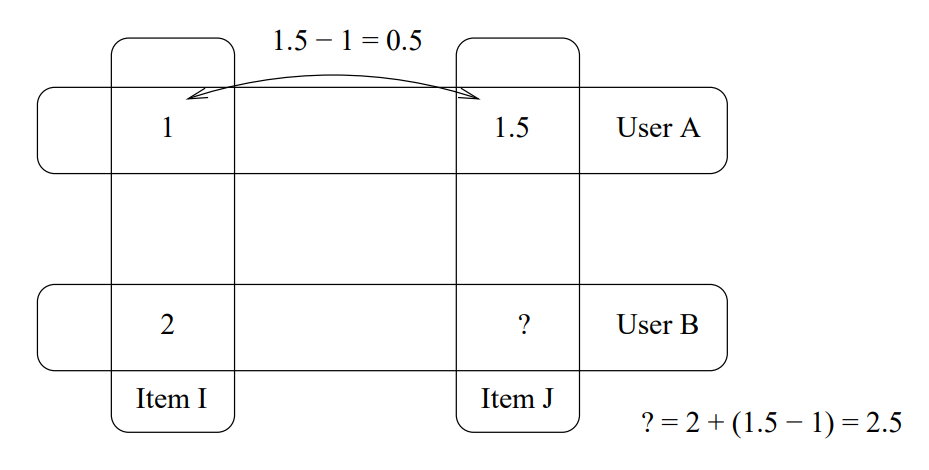
\includegraphics[keepaspectratio]{figures/algorithms/slope_one.PNG}
    \caption{Base dello schema Slope One: le valutazioni dello \textit{user} A di due \textit{item} e la valutazione  dello \textit{user} B di un \textit{item} comune vengono utilizzate per prevedere la valutazione sconosciuta dello \textit{user}.}
    \label{fig:slopeone}
\end{figure}

L'algoritmo soffre anche di diverse problematiche:
\begin{itemize}
    \item sparsità dei dati: le formule presentate prima sono approssimate considerando un dataset non sparso. Nel caso di matrici molto sparse l'algoritmo non sarà in grado di fare previsioni accurate
    \item scalabilità limitata su dataset molto grandi: la memoria necessaria per memorizzare le differenze medie dei \textit{rating} può aumentare rapidamente
    \item non tiene conto nè di personalizzazioni per \textit{user} 
    \item difficoltà a gestire grandi variazioni nelle valutazioni degli utenti
\end{itemize}

L'approccio può essere esteso a modelli ponderati e versioni più avanzate, come per esempio \textit{Weighted Slope One}, che pesa le differenze di \textit{rating} in base alla frequenza di coppie di \textit{item} valutati, e \textit{Regression-based Slope One}, che introduce funzioni non lineari per migliorare la precisione delle previsioni.

\subsection{Evaluation esplicita}\label{evaluation-esplicita}

\section{Algoritmi per il feedback implicito}\label{algoritmi-per-feedback-implicito}

\subsection{ALS (Alternating Least Squares)}\label{als}

Il lavoro di Hu, Koren e Volinsky~\cite{ALS} propone una formulazione adatta a modellare feedback impliciti, come click, acquisti o visualizzazioni.

Si basa sulla \textit{Matrix Factorization}, e una delle sue tecniche di ottimizzazione più efficaci è \textit{ALS (Alternating Least Squares)}, in particolare per dataset con \textit{feedback impliciti}.

L'obiettivo è approssimare la matrice osservata $R \in \mathbb{R}^{m \times n}$ (dove $m$ è il numero di \textit{user} e $n$ il numero di \textit{item}) come il prodotto di due matrici a bassa dimensionalità:

\[
R \approx W H^\top
\]

dove:

\begin{itemize}
    \item $W \in \mathbb{R}^{m \times k}$: matrice dei fattori latenti degli utenti,
    \item $H \in \mathbb{R}^{n \times k}$: matrice dei fattori latenti degli item,
    \item $k$: numero di fattori latenti (dimensione dello spazio latente) e iperparametro.
\end{itemize}

Si definisce la variabile binaria \textit{preferenza} $p_{ui}$ che indica la preferenza per uno \textit{user} \textit{u} per un \textit{item} \textit{i}:
\[
p_{ui} =
\begin{cases}
    1 & \text{se lo \textit{user} } u \text{ ha interagito con l'\textit{item} } i \\
    0 & \text{altrimenti}
\end{cases}
\]

e la confidenza
    
\[
c_{ui} = 1 + \alpha \cdot r_{ui}
\]
dove $r_{ui}$ in questo caso è l'interazione (es. \% visualizzazione o numero di acquisti), e $\alpha$ è un iperparametro che modula l'importanza delle osservazioni positive.

Il problema di ottimizzazione da risolvere è:

\[
\min_{W, H} \sum_{u=1}^m \sum_{i=1}^n c_{ui} (p_{ui} - w_u^\top h_i)^2 + \lambda \left( \sum_u \|w_u\|^2 + \sum_i \|h_i\|^2 \right)
\]

dove:

\begin{itemize}
    \item $w_u$: vettore dei fattori latenti per lo \textit{user} $u$,
    \item $h_i$: vettore dei fattori latenti per l' \textit{item} $i$,
\end{itemize}

Il primo termine rappresenta l'\textit{errore quadratico pesato} tra la preferenza osservata e la previsione del modello. Il secondo termine è una \textit{regolarizzazione} di tipo L2 per evitare overfitting.

Il problema in $(W,H)$ non è convesso (cioè potrebbe avere più minimi locali e non è facile trovare il minimo assoluto) ma lo diventa se si fissa una delle due variabili. Questo significa che si può trovare il minimo facilmente rispetto a $W$ tenendo $H$ fisso e viceversa. Per questo motivo, si usa un metodo iterativo finché non si arriva a una soluzione stabile:

\begin{enumerate}
    \item Si fissa $H$ e si ottimizza $W$,
    \item Si fissa $W$ e si ottimizza $H$,
    \item Si ripete per un numero prefissato di iterazioni $T$.
\end{enumerate}

Fissata $H$, per ogni \textit{user} $u$ si risolve il sistema:

\[
w_u = \left( H^\top C^u H + \lambda I \right)^{-1} H^\top C^u p^u
\]

Analogamente, per ogni \textit{item} $i$:

\[
h_i = \left( W^\top C^i W + \lambda I \right)^{-1} W^\top C^i p^i
\]

dove:

\begin{itemize}
    \item $C^u = \text{diag}(c_{u1}, \dots, c_{un})$,
    \item $p^u = (p_{u1}, \dots, p_{un})^\top$.
\end{itemize}

Il calcolo diretto dell'inversa richiede $\mathcal{O}(k^3)$ per ogni \textit{user}/\textit{item}, troppo oneroso per grandi dataset. Si può invece risolvere il sistema lineare associato:

\[
A x = b \quad \text{con} \quad A = H^\top C^u H + \lambda I, \quad b = H^\top C^u p^u
\]

utilizzando il \textit{metodo del gradiente coniugato (CG)}~\cite{ALS_opt}. Questo metodo è iterativo e richiede solo moltiplicazioni matrice-vettore, con complessità per iterazione $\mathcal{O}(k^2)$.

\begin{algorithm}[H]
    \caption{Metodo del Gradiente Coniugato per risolvere $Ax = b$}
    \begin{algorithmic}[1]
    \Require Matrice $A \in \mathbb{R}^{n \times n}$ simmetrica e definita positiva, vettore $b \in \mathbb{R}^n$, iniziale $x_0$, tolleranza $\epsilon$
    \State $r_0 \gets b - A x_0$
    \State $p_0 \gets r_0$
    \State $k \gets 0$
    \While{$\|r_k\| > \epsilon$ e $k < \text{max\_iter}$}
        \State $\alpha_k \gets \dfrac{r_k^\top r_k}{p_k^\top A p_k}$
        \State $x_{k+1} \gets x_k + \alpha_k p_k$
        \State $r_{k+1} \gets r_k - \alpha_k A p_k$
        \If{$\|r_{k+1}\| < \epsilon$}
            \State \textbf{break}
        \EndIf
        \State $\beta_k \gets \dfrac{r_{k+1}^\top r_{r+1}}{r_k^\top r_k}$
        \State $p_{k+1} \gets r_{k+1} + \beta_k p_k$
        \State $k \gets k + 1$
    \EndWhile
    \State \Return $x_{k+1}$
    \end{algorithmic}
\end{algorithm}
    
Il numero di iterazioni di \textit{GC} è un iperparametro.

Infine, lo score viene calcolato come

\[
\hat{x}_{ui} = w_u^T h_i
\]

I punti di forza dell'algoritmo sono:
\begin{itemize}
    \item efficienza computazionale: il metodo del gradiente coniugato riduce il costo computazionale rispetto all'inversione esplicita delle matrici.
    \item scalabilità: permette di gestire dataset di grandi dimensioni, grazie alla natura iterativa e alla possibilità di eseguire il calcolo in parallelo.
    \item minore uso di memoria rispetto all'inversione diretta: non è necessario costruire esplicitamente la matrice intera da invertire.
    \item velocità di convergenza: in molti casi, bastano poche iterazioni per ottenere una buona approssimazione della soluzione.
    \item supporto gpu: il calcolo iterativo si adatta bene all'accelerazione hardware, migliorando ulteriormente i tempi di addestramento.
\end{itemize}

L'algoritmo soffre anche di diverse problematiche:

\begin{itemize}
    \item approssimazione: il metodo \textit{GC} fornisce una soluzione approssimata, la cui precisione dipende dal numero di iterazioni utilizzate.
    \item sensibilità ai parametri: il numero di iterazioni (\textit{GC steps}) è un iperparametro che va scelto con attenzione per bilanciare accuratezza e prestazioni.
    \item stabilità numerica: se la matrice del sistema è mal condizionata, la convergenza del metodo \textit{GC} può essere lenta o instabile.
    \item maggiore complessità implementativa: integrare \textit{GC} richiede strutture dati e operazioni più sofisticate rispetto all'inversione diretta.
    \item overhead per piccoli dataset: su dataset piccoli, l'uso di \textit{GC} può risultare meno vantaggioso rispetto ad una soluzione esatta diretta.
\end{itemize}

\subsection{BPR (Bayesian Personalized Ranking)}\label{bpr}

Nei sistemi basati su \textit{feedback impliciti}, la mancanza di interazione tra un \textit{user} e un \textit{item} non implica necessariamente una preferenza negativa. Per affrontare tale ambiguità, BPR~\cite{BPR} adotta le seguenti ipotesi:

\begin{itemize}
    \item Se $(u, i) \in R$, cioè lo \textit{user} $u$ ha interagito con l'\textit{item} $i$, allora $u$ preferisce $i$ a tutti gli \textit{item} $j$ con cui non ha interagito.
    \item A partire da questo principio, si costruisce un insieme di triple:
    \[
    D_S := \{(u, i, j) \mid i \in I_u \wedge j \in I \setminus I_u\}
    \]
    dove ogni tripla rappresenta la preferenza dello \textit{user} $u$ per l'\textit{item} $i$ rispetto all'\textit{item} $j$.
\end{itemize}

L'obiettivo di BPR è massimizzare la probabilità a posteriori dei parametri del modello $\Theta$, dati i dati osservati:
\[
\text{BPR-Opt} = \sum_{(u, i, j) \in D_S} \ln \sigma(\hat{x}_{uij}) - \lambda_\Theta ||\Theta||^2
\]
dove:
\begin{itemize}
    \item $\hat{x}_{uij} = \hat{x}_{ui} - \hat{x}_{uj}$ è la differenza tra le valutazioni stimate per $i$ e $j$;
    \item $\sigma(x) = \frac{1}{1 + e^{-x}}$ è la funzione sigmoide;
    \item $\lambda_\Theta$ è il parametro di regolarizzazione.
\end{itemize}

Questo criterio è strettamente legato all'ottimizzazione dell'AUC (Area Under the ROC Curve), che misura la qualità del ranking.

Per prima cosa si calcola il gradiente di BPR-Opt come:

\[
\frac{\partial \text{BPR-Opt}}{\partial \Theta} =
\sum_{(u,i,j) \in D_S} 
\frac{\partial}{\partial \Theta} \ln \sigma(\hat{x}_{uij}) - 
\lambda \frac{\partial}{\partial \Theta} ||\Theta||^2
\]

\[
\propto 
\sum_{(u,i,j) \in D_S} 
\frac{-e^{-\hat{x}_{uij}}}{1 + e^{-\hat{x}_{uij}}} 
\cdot \frac{\partial}{\partial \Theta} \hat{x}_{uij} 
- \lambda \Theta
\]

L'ottimizzazione di BPR-Opt viene effettuata tramite \textit{stochastic gradient descent}. I parametri del modello sono aggirnati con:

\[
\Theta \gets \Theta - \gamma \frac{\partial \text{BPR-Opt}}{\partial \Theta}
\]


L'algoritmo effettua un campionamento \textit{bootstrap}:

\begin{algorithm}[H]
\caption{LearnBPR}
\begin{algorithmic}[1]
\Procedure{LearnBPR}{$D_S, \Theta$}
    \State Inizializza $\Theta$
    \Repeat
        \State Campiona $(u, i, j)$ da $D_S$
        \State $\Theta \gets \Theta + \gamma \cdot \left( \frac{e^{-\hat{x}_{uij}}}{1 + e^{-\hat{x}_{uij}}} \cdot \frac{\partial \hat{x}_{uij}}{\partial \Theta} - \lambda_\Theta \cdot \Theta \right)$
    \Until{convergenza}
    \State \Return $\Theta$
\EndProcedure
\end{algorithmic}
\end{algorithm}

Questo approccio consente una rapida convergenza e un buon bilanciamento tra classi positive e negative.

BPR può essere applicato a diverse famiglie di modelli. Di seguito viene presentata la versione con \textit{matrix factorization} (BPR-MF):

Ogni \textit{user} \( u \in U \) e ogni \textit{item} \( i \in I \) sono rappresentati da un vettore latente in \( \mathbb{R}^k \):

\[
\mathbf{w}_u \in \mathbb{R}^k \quad \text{(user)} \qquad
\mathbf{h}_i \in \mathbb{R}^k \quad \text{(item)}
\]


Per ogni tripla \( (u, i, j) \), il modello calcola:

\[
\hat{x}_{ui} = \langle \mathbf{w}_u, \mathbf{h}_i \rangle = \sum_{f=1}^{k} w_{uf} \cdot h_{if}
\]

\[
\hat{x}_{uj} = \langle \mathbf{w}_u, \mathbf{h}_j \rangle = \sum_{f=1}^{k} w_{uf} \cdot h_{jf}
\]

\[
\hat{x}_{uij} = \hat{x}_{ui} - \hat{x}_{uj} = \langle \mathbf{w}_u, \mathbf{h}_i - \mathbf{h}_j \rangle
\]


La funzione obiettivo da massimizzare è:

\[
\text{BPR-Opt} = \sum_{(u,i,j) \in D_S} \log \sigma(\hat{x}_{uij}) 
- \lambda \left( \|\mathbf{w}_u\|^2 + \|\mathbf{h}_i\|^2 + \|\mathbf{h}_j\|^2 \right)
\]

Definiamo:

\[
z = -\frac{\partial}{\partial \Theta} \ln \sigma(\hat{x}_{uij}) = \frac{e^{-\hat{x}_{uij}}}{1 + e^{-\hat{x}_{uij}}}
\]

Gli aggiornamenti dei parametri sono:

\begin{align*}
\mathbf{w}_u &\leftarrow \mathbf{w}_u + \gamma \left( z \cdot (\mathbf{h}_i - \mathbf{h}_j) - \lambda \cdot \mathbf{w}_u \right) \\
\mathbf{h}_i &\leftarrow \mathbf{h}_i + \gamma \left( z \cdot \mathbf{w}_u - \lambda \cdot \mathbf{h}_i \right) \\
\mathbf{h}_j &\leftarrow \mathbf{h}_j + \gamma \left( -z \cdot \mathbf{w}_u - \lambda \cdot \mathbf{h}_j \right)
\end{align*}

I punti di forza dell'algoritmo sono:

\begin{itemize}
    \item ottimizzazione diretta: massimizza la probabilità che un \textit{item} positivo sia sopra uno negativo.
    \item scalabilità: efficiente con \textit{SGD} e \textit{negative sampling}, anche su grandi dataset.
    \item flessibilità: compatibile con \textit{matrix factorization}, \textit{Neural Collaborative Filtering} e modelli più avanzati (CNN, RNN, GNN).
    \item empiricamente superiore: spesso batte metodi classici come \textit{Weighted Regularized Matrix Factorization} e \textit{SVD}\ref{svd}.
    \item indipendente da valutazioni esplicite: non richiede rating numerici.
\end{itemize}

L'algoritmo soffre anche di diverse problematiche:

\begin{itemize}
    \item negative sampling critico: la scelta degli \textit{item} negativi influisce molto sull'apprendimento.
    \item convergenza lenta: su dati sparsi può avere una convergenza lenta
    \item rischio overfitting: sensibile alla mancanza di regolarizzazione.
    \item limiti nelle relazioni globali: non cattura bene la struttura complessiva degli item.
    \item poca interpretabilità: difficile capire il motivo dietro una raccomandazione.
\end{itemize}

\subsection{LMF (Logistic Matrix Factorization)}\label{lmf-logistic-matrix-factorization}

Il modello di \textit{Logistic Matrix Factorization (LMF)}~\cite{LMF} descrive un approccio probabilistico per la fattorizzazione di matrici nel caso di feedback implicito. La probabilità che uno \textit{user} $u$ interagisca con un \textit{item} $i$ è modellata tramite una funzione logistica.

L'idea è approssimare la matrice $R$ come prodotto di due matrici più piccole:

\[
R \approx WH
\]

dove:
\begin{itemize}
    \item $W \in \mathbb{R}_{\geq 0}^{m \times k}$ rappresenta la matrice dei profili latenti degli \textit{user};
    \item $H \in \mathbb{R}_{\geq 0}^{k \times n}$ rappresenta la matrice dei profili latenti degli \textit{item};
    \item $k$ è il numero di fattori latenti e iperparametro dell'algoritmo
\end{itemize}

La probabilità che uno \textit{user} $u$ preferisca un \textit{item} $i$ è data dalla funzione logistica applicata al prodotto scalare dei fattori latenti dello \textit{user} e dell'\textit{item}, più i rispettivi bias:

\[
p(l_{ui} | w_u, h_i, \beta_u, \beta_i) = \frac{\exp(w_u^T h_i + \beta_u + \beta_i)}{1 + \exp(w_u^T h_i + \beta_u + \beta_i)}
\]

Dove:
\begin{itemize}
    \item $w_u$ è il vettore dei fattori latenti dell'\textit{user} $u$
    \item $h_i$ è il vettore dei fattori latenti dell'\textit{item} $i$
    \item $\beta_u$ è il bias dello \textit{user}
    \item $\beta_i$ è il bias dell'\textit{item}
\end{itemize}

La verosimiglianza dei dati osservati $R$ data dai parametri $W$, $H$, e $\beta$ è espressa come segue:

\[
L(R \mid W, H, \beta) = \prod_{u, i} p(l_{ui} \mid w_u, h_i, \beta_u, \beta_i)^{\alpha r_{ui}} 
\left( 1 - p(l_{ui} \mid w_u, h_i, \beta_u, \beta_i) \right)^{(1 - \alpha r_{ui})}
\]

Dove $\alpha$ è un iperparametro che bilancia il peso tra le osservazioni positive e negative.

La funzione di verosimiglianza descrive la probabilità complessiva del modello dato il comportamento osservato. In altre parole, misura quanto bene il modello spiega $R$.

Per evitare l'overfitting, si impone una distribuzione gaussiana a media zero sui vettori latenti degli utenti e degli oggetti:

\[
p(W \mid \sigma^2) = \prod_u N(w_u \mid 0, \sigma_u^2 I), \quad 
p(H \mid \sigma^2) = \prod_i N(h_i \mid 0, \sigma_i^2 I)
\]

Dove $\sigma_u^2$ e $\sigma_i^2$ sono i parametri di varianza per le distribuzioni degli utenti e degli oggetti.

L'obiettivo del modello è massimizzare il logaritmo della funzione di verosimiglianza (log-likelihood), che è dato da:

\[
\log p(W, H, \beta \mid R) = \sum_{u,i} \alpha r_{ui} (w_u^T h_i + \beta_u + \beta_i) 
- (1 + \alpha r_{ui}) \log(1 + \exp(w_u^T h_i + \beta_u + \beta_i)) 
- \lambda \|w_u\|^2 - \lambda \|h_i\|^2
\]


Il termine di regolarizzazione $\lambda$ aiuta a prevenire l'overfitting, penalizzando la grandezza dei vettori latenti.

Per ottimizzare la funzione obiettivo, vengono calcolati i gradienti parziali rispetto ai fattori latenti $w_u$ e $h_i$ e ai bias $\beta_u$ e $\beta_i$, come segue:

\[
\frac{\partial}{\partial w_u} \log p(W, H, \beta \mid R) = 
\sum_i \alpha r_{ui} h_i 
- \frac{h_i (1 + \alpha r_{ui}) \exp(w_u^T h_i + \beta_u + \beta_i)}{1 + \exp(w_u^T h_i + \beta_u + \beta_i)} 
- \lambda w_u
\]

\[
\frac{\partial}{\partial \beta_u} \log p(W, H, \beta \mid R) = 
\sum_i \alpha r_{ui} 
- \frac{(1 + \alpha r_{ui}) \exp(w_u^T h_i + \beta_u + \beta_i)}{1 + \exp(w_u^T h_i + \beta_u + \beta_i)}
\]

L'ottimizzazione avviene alternando l'ottimizzazione dei fattori latenti prima per gli \textit{user} e poi degli \textit{item}. 

Per migliorare la velocità di convergenza, viene utilizzato l'algoritmo \textit{AdaGrad} per aggiornare i parametri, adattando il tasso di apprendimento in base alla somma dei gradienti passati:

\[
w_u^t = w_u^{t-1} + \gamma \frac{g_u^{t-1}}{\sqrt{\sum_{t'=1}^t (g_u^{t'})^2}}
\]


Dove $g_u^{t-1}$ è il gradiente calcolato all'iterazione precedente e $\gamma$ è il passo di apprendimento.

Infine lo score per la coppia \textit{user} $u$ e \textit{item} $i$ si calcola come:

\[
\hat{x}_{ui} = \sigma(w_u^T h_i + \beta_u + \beta_i)
\]

I punti di forza dell'algoritmo sono:

\begin{itemize}
    \item migliore qualità e velocità di convergenza: l'utilizzo di \textit{AdaGrad} permette di migliorare e velocizzare la convergenza grazie ad una regolazione automatica dei \textit{learning rate} per ogni parametro
    \item scalabilità e semplicità: il metodo è adatto per grandi dataset e facilmente implementabile, senza la necessità di configurare iperparametri complessi
    \item modello probabilistico: LMF prevede le preferenze degli \textit{user} in modo probabilistico, il che lo rende interpretabile e facile da usare
\end{itemize}

L'algoritmo soffre anche di diverse problematiche:

\begin{itemize}
    \item complessità computazionale: nonostante sia scalabile, l'allenamento del modello su grandi dataset può richiedere una notevole potenza computazionale, specialmente con un alto numero di fattori latenti.
    \item sensibilità alla scelta dei parametri: il modello è molto dipendente dagli iperparametri, come il \textit{learning rate} e la regolarizzazione
\end{itemize}

\subsection{Evaluation implicita}\label{evaluation-implicita}

\section{Algoritmi per la similarità item-item}\label{algoritmi-per-la-similarita-item-item}

\section{Algoritmi ibridi}\label{algoritmi-ibridi}

\subsection{LightFM}\label{lightfm}

\section{Introduzione a modelli di Deep Learning}\label{introduzione-a-modelli-di-deep-learning}
